\documentclass[12pt,twoside,a4paper]{article}
\usepackage[T1]{fontenc}
\usepackage[utf8]{inputenc}
\usepackage[top=20mm, head=6mm, headsep=6mm, foot=6mm, bottom= 15mm, left=35mm, right=35mm]{geometry}
\usepackage{amsmath}
\usepackage{pythontex}
\usepackage{palatino}
\usepackage{graphicx}
\parindent0ex
\parskip2ex
\newenvironment{question}{\par\bigskip\textbf{Quesito.\kern0.2ex}}{\vspace{\parskip}}
\newenvironment{answer}{\par\bigskip\textbf{Risposta.\kern0.2ex}}{}

\pagestyle{empty}

\begin{document}



\begin{pycode}
from numpy import linspace
from numpy import log
from numpy import exp
from matplotlib.pyplot import figure, savefig, ylim, gca, plot, axis
from matplotlib import rc
rc('text', usetex=True)
rc('font', family='serif', serif='Times', size=16)
f = figure( figsize=(8,5) )
axis('off')
r = 1
k = 100
a = k/(2*exp(1))
m = r * k/exp(1)
def f( x, k=k, r=r ):
    return - r*x*log(x/k)

x   = linspace( 0.1, k*1.1 , 200 )


plot( x,f(x) )
plot( [0,k/exp(1)], [m,m] ,  color='blue', linestyle='dashed')
plot( [k/exp(1),k/exp(1)], [0,m], color='blue', linestyle='dashed')
plot(  [-3,k*1.2], [0,0], color='black')
plot(  [0,0], [-2,m*1.35], color='black')
plot( [a,a], [0,f(a)], color='blue', linestyle='dashed')
plot( [0,a], [f(a),f(a)], color='blue', linestyle='dashed')

gca().annotate(r'$\frac{rK}{e}$', 
                    xy=(-3,m), 
                    color='blue', 
                    horizontalalignment='right',  
                    verticalalignment='center')
                    
gca().annotate(r'$-r\,a\ln\!\big(\frac{a}{K}\big)$', 
                    xy=(-3,f(a)), 
                    color='blue', 
                    horizontalalignment='right',  
                    verticalalignment='center')
gca().annotate(r'$K/e$', 
                    xy=(k/exp(1),-3), 
                    color='blue', 
                    horizontalalignment='center',  
                    verticalalignment='top')
gca().annotate(r'$K$', 
                    xy=(k,-3), 
                    color='blue', 
                    horizontalalignment='center',  
                    verticalalignment='top')
                    
gca().annotate(r"$\displaystyle x'\ =\ - r\,x\,\ln\left(\frac{x}{K}\right)$", 
                    xy=(k*0.7,m), 
                    color='blue', 
                    horizontalalignment='left',  
                    verticalalignment='top') 
                    
gca().annotate(r'$0$', 
                    xy=(0,-3), 
                    color='blue', 
                    horizontalalignment='center',  
                    verticalalignment='top')        
           
gca().annotate(r"$x$", 
                    xy=(k*1.2,-1), 
                    color='blue', 
                    horizontalalignment='center',  
                    verticalalignment='top')                   
 
gca().annotate(r"$x'$", 
                    xy=(-3,m*1.35), 
                    color='blue', 
                    horizontalalignment='center',  
                    verticalalignment='top')
gca().annotate(r'$a$', 
                    xy=(a,-2), 
                    color='blue', 
                    horizontalalignment='center',  
                    verticalalignment='top')             
                    
                    
savefig('logistica1.pdf',bbox_inches='tight')
\end{pycode}

\begin{question}
L'equazione differenziale $\displaystyle x'\ =\ - r\,x\,\log\left(x/K\right)$ è una delle equazioni fenomenologiche proposte per descrivere la crescita dei tumori ($x$ rappresenta la massa).

1. Dei punti segnati nel grafico quali sono punti di equilibrio.\\
2. Dire se si tratta di equilibrio stabile o instabile.\\
3. Nei casi in cui la massa iniziale è $a$, $K/e$, $K$. Dire a quale valore tende la massa in un tempo lungo.

\hfil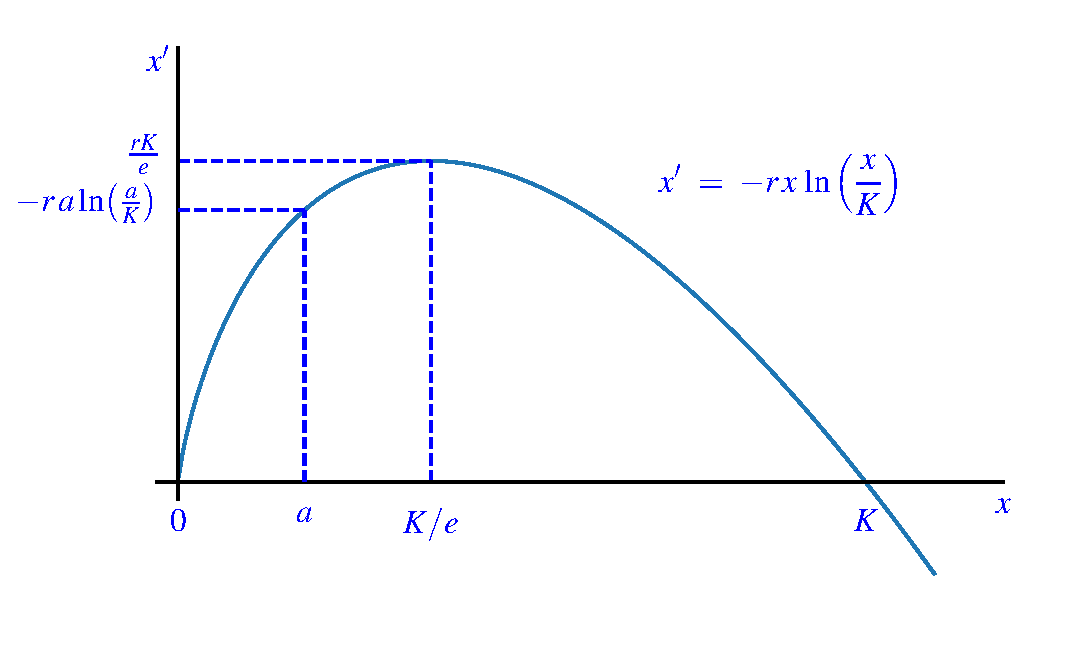
\includegraphics[width=0.9\textwidth]{logistica1.pdf}

\begin{answer}
$0$ è punto di equilibrio instabile, $K$ è punto di equilibrio stabile. In tutti e tre i casi $x(0)=a, K/e, K$ il sistema tende verso $K$.


\end{answer}
\end{question}





\begin{pycode}
from numpy import linspace
from matplotlib.pyplot import figure, savefig, ylim, gca, plot, axis
from matplotlib import rc
rc('text', usetex=True)
rc('font', family='serif', serif='Times', size=20)
f = figure( figsize=(8,5) )
axis('off')
r = 1
k = 100
h1 = 35
h2 = 15
m = r * k / 4
def f( x, k=k, r=r ):
    return r*x*(1-x/k)

x   = linspace( 0, k , 200 )

i = 0
while f( x[i] ) < h2  : 
    i += 1
    
a = x[i]
b = k - a

plot( x,f(x) )
plot( [0,k], [h1,h1], color='red',)
plot( [0,k], [h2,h2], color='green',)
plot( [0,k], [m,m] ,  color='blue',)
plot( [a,a], [0,h2], color='green', linestyle='dashed')
plot( [b,b], [0,h2], color='green', linestyle='dashed')
plot( [k/2,k/2], [0,m], color='blue', linestyle='dashed')
plot(  [0,k*1.2], [0,0], color='black')
plot(  [0,0], [0,m*1.5], color='black')

gca().annotate(r'$$r\,x\,\left(1-\frac{x}{K}\right)$$', 
                    xy=(k,h2-5), 
                    color='blue', 
                    horizontalalignment='left',  
                    verticalalignment='center')
gca().annotate(r'$H_1$', 
                    xy=(-3,h1), 
                    color='red', 
                    horizontalalignment='right',  
                    verticalalignment='center')
gca().annotate(r'$H_2$', 
                    xy=(-3,h2), 
                    color='green', 
                    horizontalalignment='right',  
                    verticalalignment='center')
gca().annotate(r'$$\frac{rK}{4}$$', 
                    xy=(-3,m), 
                    color='blue', 
                    horizontalalignment='right',  
                    verticalalignment='center')
gca().annotate(r'$K/2$', 
                    xy=(k/2,-1), 
                    color='blue', 
                    horizontalalignment='center',  
                    verticalalignment='top')
gca().annotate(r'$a$', 
                    xy=(a,-1), 
                    color='green', 
                    horizontalalignment='center',  
                    verticalalignment='top')
gca().annotate(r'$b$', 
                    xy=(b,-1), 
                    color='green', 
                    horizontalalignment='center',  
                    verticalalignment='top')
gca().annotate(r'$K$', 
                    xy=(k,-1), 
                    color='blue', 
                    horizontalalignment='center',  
                    verticalalignment='top')
gca().annotate(r'$0$', 
                    xy=(0,-1), 
                    color='blue', 
                    horizontalalignment='center',  
                    verticalalignment='top')

savefig('harvest.pdf',bbox_inches='tight')
\end{pycode}

\begin{question}
Consideriamo la seguente equazione differenziale. 

\hfil$\displaystyle\frac{{\rm d}x}{{\rm d}t}\ =\ r\,x\,\left(1-\frac{x}{K}\right) - H$

Per i tre diversi valori di $H$ rappresentati in figura $\{H_1, rK/4, H_2\}$ si dica quali dei punti sul grafico è un punto di equilibrio e se si tratta di equilibrio stabile o instabile.


\hfil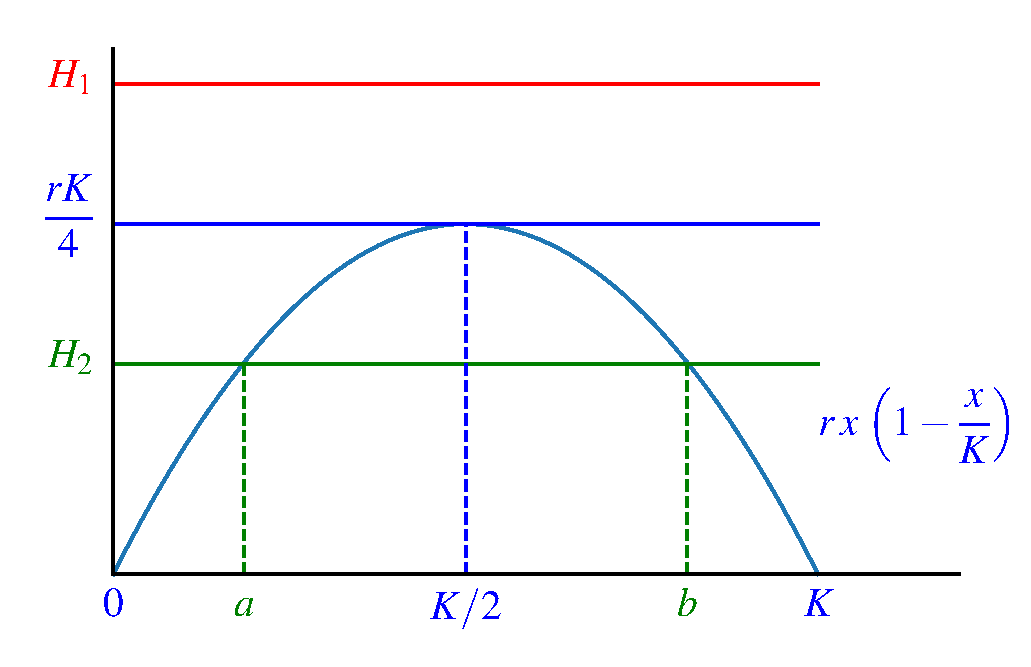
\includegraphics[width=0.9\textwidth]{harvest.pdf}
\end{question}



\begin{pycode}
from numpy import linspace
from matplotlib.pyplot import figure, savefig, ylim, gca, plot, axis
from matplotlib import rc
rc('text', usetex=True)
rc('font', family='serif', serif='Times', size=20)
f = figure( figsize=(8,5) )
axis('off')
r = 1
k = 100
a = 15
h1 = 35
h2 = 15
m = r * k / 4
def f( x, k=k, r=r ):
    return r*x*(1-x/k)*(x/a-1)

x   = linspace( 0, k , 200 )

i = 0
while f( x[i] ) < h2  : 
    i += 1
    
a = x[i]
b = k - a

tt = ((k**2-a*k+a**2)**(1/2)+k+a)/3



plot( x,f(x) )
plot(  [0,k*1.2], [0,0], color='black')
plot(  [0,0], [0,m*1.5], color='black')
plot( [tt,tt], [0,f(tt)], color='green', linestyle='dashed')

gca().annotate(r'$\frac{\sqrt{K^2-AK+A^2}+K+A}{3}$', 
                    xy=(tt,-2), 
                    color='green', 
                    horizontalalignment='center',  
                    verticalalignment='top')
gca().annotate(r'$A$', 
                    xy=(a,-1.5), 
                    color='green', 
                    horizontalalignment='center',  
                    verticalalignment='top')
gca().annotate(r'$y$',
                    xy=(k*1.2,-0.5), 
                    color='black', 
                    horizontalalignment='center',  
                    verticalalignment='top')
gca().annotate(r'$y^\prime$', 
                    xy=(-3,m*1.5), 
                    color='black', 
                    horizontalalignment='center',  
                    verticalalignment='top')
gca().annotate(r'$K$', 
                    xy=(k,-1.5), 
                    color='green',
                    horizontalalignment='center',  
                    verticalalignment='top')
gca().annotate(r'$0$', 
                    xy=(0,-1.5), 
                    color='green', 
                    horizontalalignment='center',  
                    verticalalignment='top')

savefig('Allee.pdf',bbox_inches='tight')
\end{pycode}



\begin{question}
There are populations whose rate of change over time will be negative if the population is too small (aggregation can improve the survival rate of individuals, and that cooperation may be crucial in the overall evolution of social structure). This is known as the Allee effect and can be modeled using the differential equation

\hfil$\displaystyle y^\prime\ =\ r\, y\, \left( \frac{y}{A} - 1 \right) \left( 1 - \frac{y}{K} \right)$

where $A<K$ is a constant called the Allee critical point.

Dei punti segnati nel grafico quali sono punti di equilibrio?
Dire se si tratta di equilibrio stabile o instabile.

\hfil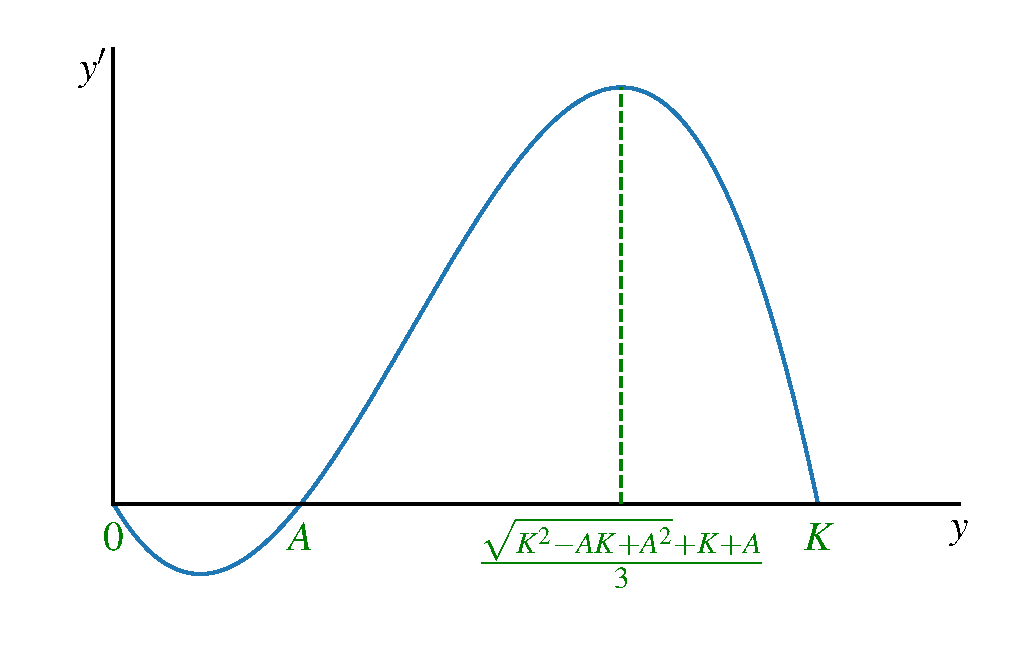
\includegraphics[width=0.9\textwidth]{Allee.pdf}

\begin{answer}
$0$ ad $A$ sono punti di equilibrio instabile, $K$ è punto di equilibrio stabile.


\end{answer}
\end{question}


\end{document}
